%   ##
%
%   Band VIII, 3 N.~??A10.6
%   Signatur/Tex-Datei: LH_35_09_15_016-017
%   RK-Nr. 41152 [Teil 6]
%   Überschrift: Tentaminum de chordarum tensione scheda sexta
%   Datierung: 1680.12.10
%   WZ: 8-blättrige Rosette auf Zahl 80 (RK-WZ: 138)
%.  SZ: groesser.png; kleiner.png (insgesamt zwei)
%.  Bilddateien (PDF): LH_35_09_15_016-017_d1; LH_35_09_15_016-017_d2; LH_35_09_15_016-017_d3 (insgesamt drei)
%
%
\begin{ledgroupsized}[r]{120mm}
\footnotesize
\pstart
\noindent\textbf{Überlieferung:}
\pend
\end{ledgroupsized}
\begin{ledgroupsized}[r]{114mm}
\footnotesize
\pstart \parindent -6mm
\makebox[6mm][l]{\textit{L}}%
Aufzeichnung: LH~XXXV~9,~15 Bl.~16\textendash17.
Ein Bogen 4\textsuperscript{o};
ein Wasserzeichen im Falz. % Achtblättrige Rosette auf Zahl 80 (RK-WZ: 138) . 
Vier einspaltig beschriebene Seiten.
% Zahlreiche Streichungen, Ergänzungen und Ersetzungen.
Die Textträger von N.~8\textsubscript{6} und N.~8\textsubscript{4} bildeten ursprünglich einen Folio-Bogen.
\pend
\end{ledgroupsized}
%
%
\vspace*{4mm}
\pstart%
\normalsize%
\noindent%
%
\lbrack16~r\textsuperscript{o}\rbrack\ % Blatt 16 r
%
\pend%
% Überschrift
\pstart%
\count\Bfootins=1500
\count\Afootins=1500
\count\Cfootins=1500
\centering%
Tentaminum\protect\index{Sachverzeichnis}{tentamen}
de chordarum tensione\protect\index{Sachverzeichnis}{tensio chordae}\\
Scheda\protect\index{Sachverzeichnis}{scheda} VI. 10 Xb. 1680
\pend%
\vspace{0.5em}%
%
\pstart%
\noindent%
Re recte expensa video me hactenus
de solis Restitutionibus omnimodis,\protect\index{Sachverzeichnis}{restitutio omnimoda}
\edtext{seu a tensione ad statum naturalem,\protect\index{Sachverzeichnis}{status naturalis}}{%
\lemma{seu}\Bfootnote{%
\hspace{-0,5mm}a tensione ad statum naturalem,
\textit{erg.~L}}}
non vero de vibrationibus
\edtext{tensorum}{%
\lemma{tensorum}\Bfootnote{\textit{erg.~L}}}
pulsatorum,
seu de restitutionibus a secunda
\edtext{tensione ad}{%
\lemma{tensione}\Bfootnote{%
\hspace{-0,5mm}\textbar~usque \mbox{\textit{gestr.}}~\textbar\ ad~%
\textit{L}}}
primam, aliquod momenti\protect\index{Sachverzeichnis}{momentum} cujusdam demonstrasse.
% \newline%
%
% \indent%
Nunc de istis cogitabo.
\pend%
%
\pstart%
\edtext{}{%
{\xxref{LH_35_09_15_016r_crassitiessuperflua-1}{LH_35_09_15_016r_crassitiessuperflua-2}}%
{\lemma{\hspace{-0.1mm}\textso{duae}\hspace{-0.4mm} \lbrack...\rbrack\ junctae}\Cfootnote{%
\hspace{-0.1mm}Siehe \cite{00044}H. \hspace{-0.1mm}\textsc{Fabri}, \hspace{-0.1mm}\textit{Physica}, \hspace{-0.1mm}tract. \hspace{-0.1mm}III, \hspace{-0.1mm}lib. \hspace{-0.1mm}II, \hspace{-0.1mm}prop. \hspace{-0.1mm}223; \hspace{-0.1mm}224
\hspace{-0.1mm}(Bd. \hspace{-0.1mm}II, Lyon\hspace{-0.1mm} 1670, S.~215b;\hspace{-0.1mm} 216a;\hspace{-0.1mm} 216b).}}}%
\edtext{Primum
\edtext{(1)}{%
\lemma{(1)}\Bfootnote{\textit{erg.~L}}}%
\protect\index{Sachverzeichnis}{chorda tensa}%
\protect\index{Sachverzeichnis}{vibratio chordae}%
\protect\index{Sachverzeichnis}{crassities chordae}%
\protect\index{Sachverzeichnis}{tempus vibrationis}%
\edlabel{LH_35_09_15_016r_crassitiessuperflua-1}%
\!\textso{ duae chordae sola crassitie differentes,
eodem tempore suas vibrationes absolvent,}
quia perinde est ac si plures chor\-dae essent junctae.%
\edlabel{LH_35_09_15_016r_crassitiessuperflua-2}}{%
\lemma{\textit{Am Rand:}}\Afootnote{%
abstrahendo a resistentia aeris%
\protect\index{Sachverzeichnis}{resistentia aeris}\vspace{-0.0em}}}
\pend%
%
\pstart%
\edtext{(2)}{%
\lemma{(2)}\Bfootnote{\textit{erg.~L}}}%
\protect\index{Sachverzeichnis}{chorda tensa}%
\protect\index{Sachverzeichnis}{longitudo chordae}%
\protect\index{Sachverzeichnis}{tempus vibrationis}%
\edlabel{LH35_09_15_016r_freqzulaeng-1}\textso{ Duae\! chordae\! aeque\! }%
\edtext{\textso{tensae\! longitudine\!}}{%
\lemma{\textso{tensae}}\Bfootnote{% \hspace*{-0,5mm}
\textbar~\textso{sola} \textit{gestr.}~\textbar\ \textso{longitudine}~%
\textit{L}}}%
\textso{ differentes\! habent tempora vibrationum in ratione longitudinum.}\edlabel{LH35_09_15_016r_freqzulaeng-2} % \,\,\,%
Hoc eodem modo demonstratur
in vibrationibus\protect\index{Sachverzeichnis}{vibratio chordae}
atque in restitutionibus.\protect\index{Sachverzeichnis}{restitutio chordae}
Hoc posset etiam assumi
velut hypothesis
comprobata experimento.\protect\index{Sachverzeichnis}{hypothesis comprobata experimento}
%
Est enim fundamentum\protect\index{Sachverzeichnis}{fundamentum} sectionis
\edtext{Monochordi.\protect\index{Sachverzeichnis}{sectio monochordi}
\newline%
%
\indent%
(3)\edlabel{LH_35_09_15_016r_propositio3-1}%
\protect\index{Sachverzeichnis}{chorda tensa}%
\textso{ Chordae ejusdem}}{%
\lemma{Monochordi.}\Bfootnote{%
\textit{(1)}~Duae chordae
\textit{(2)}~\textbar~(3) \textit{erg.}~\textbar\ \textso{Chordae ejusdem}%
~\textit{L}}}%
\textso{ eodem semper modo tensae }%
(\phantom)\hspace*{-1.2mm}%
adeoque et chordarum non nisi
crassitie\protect\index{Sachverzeichnis}{crassities chordae} differentium%
\phantom(\hspace*{-1.2mm})%
\textso{ vibrationes magnae pariter et}
%\pend
%\newpage
%\pstart
%\noindent 
\textso{parvae sunt isochronae.}%
\protect\index{Sachverzeichnis}{vibratio isochrona}
Hoc etiam
experimento\protect\index{Sachverzeichnis}{experimentum} comprobatur,
esset tamen
%%%%%%%%%%%%%%
\edlabel{KZeitz115}\edtext{}{{\xxref{KZeitz115}{KZeitz116}}%
{%
\lemma{demonstrandum.}\Bfootnote{%
\textit{(1)}~Chordae magis tensae, ceteris paribus vibr
\textit{(2)}~\textbar~(4) \textit{erg.}~\textbar\ \textso{Chordae}
\textit{(a)}~\textso{magis}
\textit{(b)}~\textso{ejusdem magis tensae vibrationes}%
~\textit{L}}}}%
demonstrandum.\edlabel{LH_35_09_15_016r_propositio3-2}
\pend
\newpage
\pstart
(4)%
\protect\index{Sachverzeichnis}{chorda tensa}%
\protect\index{Sachverzeichnis}{vibratio chordae}%
\textls{ Chordae ejusdem magis tensae vibrationes\edlabel{KZeitz116} sunt celeriores.}
Hoc etiam
constat experimento,\protect\index{Sachverzeichnis}{experimentum}
sed et ratione.\protect\index{Sachverzeichnis}{ratio}
\pend%
\count\Bfootins=1000
\count\Afootins=1000
\count\Cfootins=1000
%
\pstart%
\edtext{(5)}{%
\lemma{(5)}\Bfootnote{%
\textit{erg.~L}}}%
\protect\index{Sachverzeichnis}{chorda tensa}%
\protect\index{Sachverzeichnis}{tensio chordae}%
\protect\index{Sachverzeichnis}{crassities chordae}%
\textls{ Si duae sint chordae sola tensione et forte crassitie differentes,
magis tensa vibrationes habet celeriores.}%
\protect\index{Sachverzeichnis}{vibratio chordae}
Hoc etiam
experimento\protect\index{Sachverzeichnis}{experimentum}
et ratione\protect\index{Sachverzeichnis}{ratio} manifestum
\edtext{est.
\newline%
%
\indent%
(6)\edlabel{LH_35_09_15_016r_iisdemquaeantea-1} 
Si chorda $A$ a chorda $B$ minus tensa\protect\index{Sachverzeichnis}{chorda tensa}
sola tensione\protect\index{Sachverzeichnis}{tensio chordae}
(\phantom)\hspace*{-1.2mm}%
et crassitie\protect\index{Sachverzeichnis}{crassities chordae} forsan%
\phantom(\hspace*{-1.2mm})
differat,
et ab eadem chorda $B$ aeque tensa
postmodum longitudine\protect\index{Sachverzeichnis}{longitudo chordae} solum
(\phantom)\hspace*{-1.2mm}%
et forte crassitie\protect\index{Sachverzeichnis}{crassities chordae}%
\phantom(\hspace*{-1.2mm})
differat,\edlabel{LH_35_09_15_016r_iisdemquaeantea-2}}{%
\lemma{est.}\Bfootnote{%
\textit{(1)}~Sint tres ch
\textit{(2)}~Chorda $A$ a chorda $B$ solae tensionis differens,
\textit{(3)}~\textbar~(6) \textit{erg.}~%
\textbar\ Si chorda $A$ a chorda $B$
\textbar~minus tensa \textit{erg.}~%
\textbar\ sola tensione
\textbar~(\phantom)\hspace*{-1.2mm}et crassitie forsan\phantom(\hspace*{-1.2mm}) \textit{erg.}~%
\textbar\ differat, et \lbrack...\rbrack\ forte crassitie\phantom(\hspace*{-1.2mm})
\textit{(a)}~differens,
\textit{(b)}~differat,%
~\textit{L}}}
tunc chorda $B$ magis tensa celerius vibrabit quam ipsa $B$
\edtext{minus tensa,%
\textso{ per~4;}
tardius vero quam ipsa $A,$
quia ipsa $A$ est brevior et aeque tensa,\protect\index{Sachverzeichnis}{chorda tensa}%
\textso{ per 2. }}{%
\lemma{minus}\Bfootnote{%
\hspace{-0,5mm}tensa,
\textit{(1)}~tardius tamen
\textit{(2)}~per precedentem;
\textit{(3)}~\textso{per 4;} \lbrack...\rbrack\ \textso{per 2.}%
~\textit{L}}}%
\!Seu%
\textso{ chorda magis tensa mediae est celeritatis inter seipsam minus tensam,
et aliam ipsi minus tensae longitudine,
et magis tensae tensione }%
\protect\index{Sachverzeichnis}{chorda tensa}%
\protect\index{Sachverzeichnis}{celeritas vibrationis}%
\protect\index{Sachverzeichnis}{longitudo chordae}%
\protect\index{Sachverzeichnis}{tensio chordae}%
% Sich über den Seitenumbruch erstreckende Variante : Beginn
\edtext{\textso{aequalem.}
%
\lbrack16~v\textsuperscript{o}\rbrack\ % Blatt 16 v
%
\newline%
%
\indent%
(7)
Hinc cum vibrandi tempora\protect\index{Sachverzeichnis}{tempus vibrandi}
chordae permanentis et mutabilis%
\protect\index{Sachverzeichnis}{chorda permanens}%
\protect\index{Sachverzeichnis}{chorda mutabilis}
aeque cum ipsa tensae,
seu magis quam ante tensae\protect\index{Sachverzeichnis}{chorda tensa}%
\lbrack,\rbrack\ sint
\edtext{ut longitudines,\protect\index{Sachverzeichnis}{longitudo chordae}}{%
\lemma{\textit{Am Rand, auf} ut longitudines \textit{bezogen:}}%
\Afootnote{potius ut longitudinum excessus super naturalem%
\protect\index{Sachverzeichnis}{longitudo chordae naturalis}}}
et%
\!\textso{ }%
\edtext{\textso{longitudines ejusdem chordae diversimode tensae sint ut tensiones,%
\protect\index{Sachverzeichnis}{tensio chordae}}}{%
\lemma{\textso{longitudines} \lbrack...\rbrack\ \textso{tensiones}}%
\Cfootnote{Doppelt unterstrichen.}}%
}{%
\lemma{\textso{aequalem.}}\Bfootnote{%
\textit{(1)}~Hinc cum
\textit{(a)}~chorda
\textit{(aa)}~tertia sit ad minus t
\textit{(bb)}~altera sit
\textit{(cc)}~permanens
\textit{(aaa)}~sit
\textit{(bbb)}~sit ad minus tensam
\textit{(b)}~vibrandi tempora chordae permanentis
\textit{(aa)}~et minus
\textit{(bb)}~et magis tensae sint in ratione longitudinum, 
\textit{(2)}~Hinc chord
\lbrack16~v\textsuperscript{o}\rbrack\
\textit{(3)}~Hinc cum \lbrack...\rbrack\ ipsa tensae
\textit{(a)}~sint
\textit{(b)}~,~seu magis \lbrack...\rbrack\ ut longitudines,
\textit{(aa)}~seu ut
\textit{(aaa)}~magis
\textit{(bbb)}~chordae mutabilis tensiones,
\textit{(bb)}~et \textso{longitudines}
\textit{(aaa)}~duarum chordarum aeque tensarum
\textit{(bbb)}~\textso{ejusdem chordae} \lbrack...\rbrack\ \textso{ut tensiones,}%
~\textit{L}}}
% Sich über den Seitenumbruch erstreckende Variante : Ende
et in nostro Casu
\edtext{Chorda permanens\protect\index{Sachverzeichnis}{chorda permanens}}{%
\lemma{Chorda}\Bfootnote{%
\textit{(1)}~minus tensa
\textit{(2)}~permanens%
~\textit{L}}}
longitudini minori\protect\index{Sachverzeichnis}{longitudo chordae}
\edtext{chordae mutabilis\protect\index{Sachverzeichnis}{chorda mutabilis}}{%
\lemma{chordae}\Bfootnote{%
\textit{(1)}~minoris
\textit{(2)}~mutabilis%
~\textit{L}}}
\edtext{aequalis sit,}{%
\lemma{aequalis}\Bfootnote{%
\textit{(1)}~est,
\textit{(2)}~sit,%
~\textit{L}}}
sequitur,
iisdem quae
\edtext{antea}{%
\lemma{antea}\Cfootnote{%
S.~\refpassage{LH_35_09_15_016r_iisdemquaeantea-1}{LH_35_09_15_016r_iisdemquaeantea-2}.}}
positis\lbrack,\rbrack%
\textso{ chordae }%
\edtext{\textso{permanentis et chordae mutabilis
magis quam antea tensae
tempora vibrandi esse}}{%
\lemma{\textso{permanentis}}\Bfootnote{%
\textit{(1)}~tempora vibrandi
\textit{(2)}~\textso{et chordae aeque tensae}
\textit{(3)}~\textso{et chordae} \lbrack...\rbrack\ \textso{antea tensae}
\textit{(a)}~vibrationes esse
\textit{(b)}~\textso{tempora vibrandi esse}%
~\textit{L}}}%
\textso{ ut chordae mutabilis }%
\protect\index{Sachverzeichnis}{chorda tensa}%
\protect\index{Sachverzeichnis}{tempus vibrandi}%
\protect\index{Sachverzeichnis}{chorda permanens}%
\edtext{\textso{tensiones.}\protect\index{Sachverzeichnis}{tensio chordae}
Sit chorda mutabilis $ABC,$\protect\index{Sachverzeichnis}{chorda mutabilis}}{% 
\lemma{\textso{tensiones.}}\Bfootnote{%
\textit{(1)}~Optimum erit adhibere figuras,\protect\index{Sachverzeichnis}{figura}
\textit{(2)}~Sit
\textit{(a)}~linea
\textit{(b)}~chorda
\textit{(aa)}~$AB$
\textit{(bb)}~mutabilis $ABC,$%
~\textit{L}}}
minus tensa $AB,$ magis tensa $ABC,$
et sit chorda $DE$\protect\index{Sachverzeichnis}{chorda tensa}
longitudine\protect\index{Sachverzeichnis}{longitudo chordae} aequa\-lis ipsi $AB,$
tensione\protect\index{Sachverzeichnis}{tensio chordae} aequalis ipsi $ABC.$
Erit tempus\edlabel{LH_35_09_15_016v_kjgrsejoi-1} vibrandi\protect\index{Sachverzeichnis}{tempus vibrandi} chordae $DE$
ad tempus vibrandi\protect\index{Sachverzeichnis}{tempus vibrandi} chordae $AC,$
ut\protect\index{Sachverzeichnis}{recta}
\edtext{recta $DE$ ad rectam $ABC,$\textso{ per 2,} seu}{%
\lemma{recta}\Bfootnote{%
\hspace{-0,5mm}$DE$ \textbar~vel $AB$ \textit{gestr.}~\textbar\ ad rectam $ABC,$
\textit{(1)}~vel
\textit{(2)}~\textso{per 2,} seu%
~\textit{L}}}
(\phantom)\hspace*{-1.2mm}%
quia ex hypothesi\protect\index{Sachverzeichnis}{hypothesis} $DE$ aequ. $AB$%
\phantom(\hspace*{-1.2mm})
%%%% distilletur-huomaus reunassa / alus
\edtext{}{%
{\xxref{LH_35_09_15_016v_distmarg-1}{LH_35_09_15_016v_distmarg-2}%
{\lemma{\textit{Am Rand nebst Hervorhebungszeichen:}}\Afootnote{%
\Denarius\vspace{3mm}}}}}%
ut\edlabel{LH_35_09_15_016v_distmarg-1}
recta $AB$ ad
\edtext{rectam $AC.$\edlabel{LH_35_09_15_016v_kjgrsejoi-2}\protect\index{Sachverzeichnis}{recta}
Sunt}{%
\lemma{rectam}\Bfootnote{%
\hspace{-0,5mm}$AC.$
\textit{(1)}~Sunt
\textit{(2)}~Est
\textit{(3)}~Sunt%
~\textit{L}}}
\edtext{autem $AB$ et $AC$}{%
\lemma{autem}\Bfootnote{%
\hspace{-0,5mm}$AB$
\textit{(1)}~ad
\textit{(2)}~et $AC$%
~\textit{L}}}
ut chordae mutabilis\protect\index{Sachverzeichnis}{chorda mutabilis}
\edtext{$ABC$}{%
\lemma{$ABC$}\Bfootnote{\textit{erg.~L}}}
tensiones,\protect\index{Sachverzeichnis}{tensio chordae}
per ea quae
\edtext{superius}{%
\lemma{superius}\Cfootnote{%
Siehe N.~8\textsubscript{2}, S.~\refpassage{LH_35_09_15_009r_tensutlong-1}{LH_35_09_15_009r_tensutlong-2}.}}
sunt
\edtext{demonstrata.\edlabel{LH_35_09_15_016v_distmarg-2}
%%%% distilletur-huomaus reunassa / loppu
Ergo chordae permanentis $DE$\protect\index{Sachverzeichnis}{chorda permanens}
et mutabilis aeque cum ipsa tensae\protect\index{Sachverzeichnis}{chorda tensa}
tempora vibrandi\protect\index{Sachverzeichnis}{tempus vibrandi} sunt inter se,}{%
\lemma{demonstrata.}\Bfootnote{%
\textit{(1)}~Ergo su
\textit{(2)}~Ergo
\textit{(a)}~chorda permanens $DE$
\textit{(aa)}~est ad
\textit{(bb)}~habet tempus vibrandi quod est
\textit{(b)}~chordae permanentis \lbrack...\rbrack\ ipsa tensae
\textbar~tempora vibrandi \textit{erg.}~\textbar\ sunt inter se,%
~\textit{L}}}
ut tensio mutabilis aeque cum ipsa longae,
ad tensionem mutabilis aeque cum ipsa tensae,\protect\index{Sachverzeichnis}{chorda mutabilis}
seu ut mutabilis tensiones.\protect\index{Sachverzeichnis}{tensio chordae}
\pend%
%
%
  \vspace{1.5em}
  \centerline{\includegraphics[width=0.48\textwidth]{gesamttex/edit_VIII,3/images/LH_35_09_15_016-017_d1.pdf}}%\\
  \vspace{0.5em}%
  \centerline{\lbrack\textit{Fig.~1}\rbrack}%
  \vspace{1.4em}%
%  \newpage% Rein vorläufig !!!!
%
%
\pstart%
(8)
\edtext{Hinc cum $AB$ exprimat tempus
vibrandi\protect\index{Sachverzeichnis}{tempus vibrandi}
chordae $DE,$}{%
\lemma{Hinc}\Bfootnote{%
\textit{(1)}~si
\textit{(2)}~chorda mutabilis
\textit{(3)}~cum $AB$ exprimat tempus vibrandi
\textit{(a)}~chordae
\textit{(b)}~chordae
\textit{(aa)}~unitat
\textit{(bb)}~$DE,$%
~\textit{L}}}
et $AC$ tempus vibrandi chordae $AC,$
et vero chorda $AB$ tardius ad hoc vibretur quam $AC$%
\textso{ per 4,}
ergo producta $AC$ aliquousque in $\beta,$
ipsa $AB$ exprimet vibrationem chordae $AB$.\protect\index{Sachverzeichnis}{vibratio chordae}
Hinc%
\textso{ chordae diversimodae tensae }%
\protect\index{Sachverzeichnis}{chorda diversimode tensa}%
\edtext{(\phantom)\hspace{-0.5mm}$AB.$ $AC$\phantom(\hspace{-0.5mm})}{%
\lemma{(\phantom)\hspace{-1.2mm}$AB.$}\Bfootnote{%
\hspace{-1mm}$AC$\phantom(\hspace{-1.2mm}) \textit{erg.~L}}}%
\hspace{0.3mm}\textso{ tempus vibrandi in minore tensione }
%-}
%\pend
%\newpage
%\pstart
%\noindent
%\textso{sione }%
\protect\index{Sachverzeichnis}{tensio chordae}%
($AB$)%
\textso{ est ad tempus }%
\protect\index{Sachverzeichnis}{tempus vibrandi}%
\protect\index{Sachverzeichnis}{chorda mutabilis}%
\protect\index{Sachverzeichnis}{tensio chordae}%
\protect\index{Sachverzeichnis}{longitudo chordae}%
\edtext{\textso{vibrandi chordae $DE$ tensione mutabilem magis tensam $AC\!$,
longitudine minus tensam $AB$ aequantis }}{%
\lemma{\textso{vibrandi}}\Bfootnote{%
\textit{(1)}~in majore tensione, $AC$
\textit{(2)}~\textso{chorda}
\textit{(3)}~\textso{chorda $DE$ tensione}
\textbar~\textso{mutabilem} \textit{erg.}~\textbar\ \textso{magis}
\textit{(a)}~\textso{tensae}
\textit{(b)}~\textso{tensam $AC,$} \lbrack...\rbrack\ \textso{$AB$ aequantis}%
~\textit{L}}}%
(\phantom)\hspace*{-1.2mm}%
seu $A\beta$ est ad $AB$%
\phantom(\hspace*{-1.2mm})%
\textso{ in ratione majore quam reciproca }%
\edtext{\textso{tensionum}%
\protect\index{Sachverzeichnis}{tensio chordae}%
\textso{ seu reciproca longitudinum,}%
\protect\index{Sachverzeichnis}{longitudo chordae}
(\phantom)\hspace*{-1.2mm}%
seu in majore ratione}{%
\lemma{\textso{tensionum}}\Bfootnote{%
\textit{(1)}~(\phantom)\hspace*{-1.2mm}seu in majore ratione
\textit{(2)}~\textso{seu reciproca} \lbrack...\rbrack\ majore ratione%
~\textit{L}}}
quam $AC$ ad $AB,$%
\lbrack\phantom(\hspace*{-1.2mm})\rbrack\
\edtext{seu%
\textso{ duae chordae sola tensione }%
\protect\index{Sachverzeichnis}{tensio chordae}%
(\phantom)\hspace*{-1.2mm}%
et forte crassitie%
\protect\index{Sachverzeichnis}{crassities chordae}%
\phantom(\hspace*{-1.2mm})%
\textso{ }%
\edtext{\textso{differentes }$AB.$ $DE$\textso{ habent tempora vibrandi in ratione}%
\protect\index{Sachverzeichnis}{tempus vibrandi}}{%
\lemma{\textso{differentes}}\Bfootnote{%
\textit{(1)}~habent tem
\textit{(2)}~$AB.$ $DE$ \textso{habent tempora vibrandi}
\textit{(a)}~in ratione
\textit{(b)}~\textso{in ratione}
~\textit{L}}}%
\textso{ }%
(\phantom)\hspace*{-1.2mm}%
$A\beta$ ad $AB$%
\phantom(\hspace*{-1.2mm})%
\textso{ majore quam }%
(\phantom)\hspace*{-1.2mm}%
$AC$ ad $AB$%
\phantom(\hspace*{-1.2mm})%
\textso{ reciproca tensionum }%
\edtext{(\phantom)\hspace*{-1.2mm}%
nempe linea $AC$ repraesentans tensionem ipsius chordae $DE,$
et linea $AB$ vel $DE$ tensionem ipsius chordae $AB$%
\protect\index{Sachverzeichnis}{tensio chordae}%
\phantom(\hspace*{-1.2mm})
seu}{%
\lemma{(\phantom)\hspace*{-1.2mm}nempe}\Bfootnote{%
\hspace{-0,6mm}\textbar~linea \textit{erg.}~%
\textbar\ $AC$ repraesentans tensionem ipsius
\textbar~chordae \textit{erg.}~%
\textbar\ $DE,$ et
\textbar~linea \textit{erg.}~%
\textbar\ $AB$
\textbar~vel $DE$ \textit{erg.}~%
\textbar\ tensionem ipsius
\textbar~chordae \textit{erg.}~%
\textbar\ $AB$\phantom(\hspace*{-1.2mm}) seu~%
\textit{L}}}%
\textso{ habent celeritates vibrandi in ratione majore quam tensionum.}%
\protect\index{Sachverzeichnis}{celeritas vibrandi}%
\protect\index{Sachverzeichnis}{tensio chordae}%
}{\lemma{\textit{Am Rand}}\Afootnote{\textit{\hspace*{-0,4mm}Hervorhebungszeichen}}}
%
\lbrack17~r\textsuperscript{o}\rbrack\ % Blatt 17 r
%
\pend%
\count\Bfootins=1000
\count\Afootins=1200
\count\Cfootins=1000
%\newpage
\pstart%
\edlabel{KZeitz97}\edtext{}%
{{\xxref{KZeitz97}{KZeitz98}}%
{\lemma{\textit{Am Rand:}}\Afootnote{%
Pro vero habeo,%
\textsuperscript{[a]} %
unam chordam diversimode tensam\protect\index{Sachverzeichnis}{chorda diversimode tensa}
habere%
\textsuperscript{[b]} %
vibrationes\protect\index{Sachverzeichnis}{vibratio chordae}
seu tonos\protect\index{Sachverzeichnis}{tonus}
in ratione tensionum,\protect\index{Sachverzeichnis}{tensio chordae}
sive virium tendentium;\protect\index{Sachverzeichnis}{vis tendens}
sed tunc \protect\rule[-1.8mm]{0mm}{0mm}supponendum est%
\textsuperscript{[c]} %
eam habere longitudinem\protect\index{Sachverzeichnis}{longitudo chordae quaesita}
tensione nova\protect\index{Sachverzeichnis}{tensio nova} quaesitam.
Nam si priorem longitudinem retinet,\protect\index{Sachverzeichnis}{longitudo chordae prior}
non sunt \lbrack unius\rbrack%
\textsuperscript{[d]} %
\protect\rule[-1.6mm]{0mm}{0mm}chordae diversi status,\protect\index{Sachverzeichnis}{status chordae}
sed duae chordae aeque longae sola tensione differentes.
\protect\rule[-1.2mm]{0mm}{0mm}Et hoc fit cum chorda $AB$ tendatur pondere $D.$\protect\index{Sachverzeichnis}{pondus tendens}
Nam duplo pondere appenso\protect\index{Sachverzeichnis}{pondus appensum} quam ante\lbrack,\rbrack\
$AB$ prior \protect\rule[-1.6mm]{0mm}{0mm}et $AB$ posterior sunt duae chordae
sola tensione differentes,\protect\index{Sachverzeichnis}{tensio chordae}
unde mirum non est celeritates\protect\index{Sachverzeichnis}{celeritas vibrandi}
\protect\rule[-1.6mm]{0mm}{0mm}esse in duplicata ratione\textsuperscript{[e]} tensionum,
seu duplicatis ponderibus tonum esse quadruplo acutiorem.%
\protect\index{Sachverzeichnis}{tonus acutus}%
\vspace{1.0em}%
%%\\%
\\%
\centerline{\protect\includegraphics[width=0.28\textwidth]{gesamttex/edit_VIII,3/images/LH_35_09_15_016-017_d2.pdf}}%
\\
\centerline{\lbrack\textit{Fig.~2}\rbrack}%
\\%
\\%
\footnotesize{%
%%%%
\textsuperscript{[a]}~%
habeo,
\textit{(1)}~duas
\textit{(2)}~unam%
~\textit{L}
\quad
%%%%
\textsuperscript{[b]}~%
habere
\textit{(1)}~tensionem
\textit{(2)}~vibrationes seu tonos%
~\textit{L}
\quad
%%%%
\textsuperscript{[c]}~%
est
\textit{(1)}~quoque retinere eam
\textit{(2)}~eam habere%
~\textit{L}%
\quad
%%%%
\textsuperscript{[d]}~%
duae
\textit{L ändert Hrsg.}
%
\quad
%%%%
\textsuperscript{[e]}~%
duplicata ratione:
Es gilt um\-ge\-kehrt, dass die Frequenz sich wie die Quadratwurzel der Spannkraft verhält, weshalb das vierfache Gewicht nötig ist, um eine Saite mit doppelter Frequenz schwingen zu lassen.
Siehe etwa \cite{01227}M.~\textsc{Mersenne}, \textit{Ballistica}, prop.~36 (Paris 1644, S.~128\textendash132) sowie Leibnizens Randbemerkung in N.~8\textsubscript{4}, S.~\refpassage{LH_35_09_15_013r_widerlegung-2}{LH_35_09_15_013r_widerlegung-2}.%\vspace{-1.5em}%
}%
}}}%
% Ende der Marginalie
(9)
Hinc%
\protect\index{Sachverzeichnis}{tensio chordae}%
\textso{ si duae chordae sola tensione differentes }%
\edtext{$AB.$ $DE$\textso{ haberent}}{%
\lemma{$AB.$}\Bfootnote{%
\hspace{-0,5mm}$DE$
\textit{(1)}~\textso{habuerint}
\textit{(2)}~\textso{haberent}%
~\textit{L}}}%
\protect\index{Sachverzeichnis}{celeritas vibrandi}%
\textso{ celeritates in ratione majore vel minore quam duplicata tensionum,}
(\phantom)\hspace*{-1.2mm}%
%\protect\rule[-4mm]{0mm}{6mm}%
seu si $A\beta$ \!:\! $AB$
$\!\displaystyle\kleiner\!$
vel
$\!\displaystyle\groesser\!$ $\displaystyle\squaredots$
$CA\!$ quadr. \!:\!
\edtext{$BA\!$ quadr.% 
\phantom(\hspace*{-1.2mm})%
\textso{ tunc}}{%
\lemma{$BA$}\Bfootnote{%
\hspace{-0,5mm}quadr.
\textbar~seu si $\beta A$ \!:\! $CA$ $\!\displaystyle\efrac{\ggroesser}{\kkleiner}\!$ $CA$ \!:\! $BA$
\textit{erg.~u. gestr.}~%
\textbar~\phantom(\hspace*{-1.2mm}) \textso{tunc}%
~\textit{L}}}%
\textso{ ejudsem chordae} \makebox[1.0\textwidth][s]{\textso{diversi status }%
\protect\index{Sachverzeichnis}{status chordae}%
\edtext{(\phantom)\hspace*{-1.2mm}$AB.$ $AC$\phantom(\hspace*{-1.2mm})\textso{ habebunt}}{%
\lemma{(\phantom)\hspace*{-1.2mm}$AB.$}\Bfootnote{%
\hspace*{-0,5mm}$AC$\phantom(\hspace*{-1.2mm})
\textit{(1)}~\textso{haberent}
\textit{(2)}~\textso{habebunt}%
~\textit{L}}}%
\textso{ celeritates }%
\protect\index{Sachverzeichnis}{celeritas vibrandi}%
\edtext{\textso{etiam in ratione majore}}{%
\lemma{\textso{etiam}}\Bfootnote{%
\textit{(1)}~majore
\textit{(2)}~\textso{in ratione majore}%
~\textit{L}}}}%
%\protect\rule[0pt]{0mm}{14pt}%
%\textso{ vel}
\pend
\newpage
\pstart
\noindent \textso{vel minore }%
\edtext{\textso{quam simplici tensionum }%
\protect\index{Sachverzeichnis}{tensio chordae}%
et contra
(\phantom)\hspace*{-1.2mm}seu erunt $\beta A$}{%
\lemma{\textso{quam}}\Bfootnote{%
\textit{(1)}~\textso{tensionum}
\textit{(2)}~\textso{simplici tensionum}
\textit{(a)}~(\phantom)\hspace*{-1.2mm}seu erunt $\beta$
\textit{(b)}~et contra (\phantom)\hspace*{-1.2mm}seu erunt $\beta A$%
~\textit{L}}}
\!:\! $CA$ $\displaystyle\groesser\!$ \!vel\! $\displaystyle\kleiner\!$ $CA$ \!:\! $BA.$
%\protect\rule[0pt]{0mm}{21pt}%
Quia % $\underset{\displaystyle\ggroesser}{\kkleiner}$
\edtext{si $\beta A$ \!:\! $BA$}{%
\lemma{si}\Bfootnote{%
\textit{(1)}~$\beta\alpha$ qu
\textit{(2)}~$\beta\alpha$
\textit{(3)}~$\beta A$~:
\textit{(a)}~$AB$
\textit{(b)}~$BA$%
~\textit{L}}}
$\!\displaystyle\efrac{\ggroesser}{\kkleiner}\!$ $CA\!$ quadr. \!:\! $BA\!$ quadr.
Ergo
% \protect\rule[0pt]{0mm}{0pt}%
$\beta A$ \!:\! $CA$ $\!\displaystyle\efrac{\ggroesser}{\kkleiner}\!$ $CA$ \!:\! $BA.$%
\phantom(\hspace*{-1.2mm})\edlabel{KZeitz98}%%
\pend%
%
\count\Bfootins=1000
\count\Afootins=1000
\count\Cfootins=1000
%\newpage
\pstart%
(10) Et%
\protect\index{Sachverzeichnis}{tensio chordae}%
\textso{ si duae chordae sola tensione differentes habent celeritates in ratione duplicata }%
\protect\index{Sachverzeichnis}{celeritas vibrandi}%
\protect\index{Sachverzeichnis}{status chordae}%
\edtext{\textso{tensionum, tunc ejusdem chordae diversi status habebunt celeritates in ratione}}{%
\lemma{\textso{tensionum,}}\Bfootnote{%
\textit{(1)}~erunt
\textit{(2)}~\textso{tunc ejusdem} \lbrack...\rbrack\ \textso{status habebunt}
\textit{(a)}~chordas in ratione
\textit{(b)}~\textso{celeritates in ratione}%
~\textit{L}}}%
\textso{ ipsarum }%
\edtext{\textso{tensionum.}\protect\index{Sachverzeichnis}{tensio chordae}
Et contra, patet ex praecedenti.
\newline%
\indent%
Et si\protect\rule[0pt]{0mm}{14pt}
$\beta A$ \!:\! $CA$ $\displaystyle\groesser\!$ $CA$ \!quadr. \!\lbrack:\rbrack\! $BA$ \!quadr.
erit $\beta A$ \!:\! $BA$ $\displaystyle\groesser\!$ $CA$ \!cub. \!:\! $BA$~\!cub.~%
Et contra. Seu%
\textso{ si duae chordae}}{%
\lemma{\textso{tensionum.}}\Bfootnote{%
\textit{(1)}~Et si duae chordae
\textit{(2)}~Et contra, \lbrack...\rbrack\ : $BA$ cub.
\textbar~Et contra. \textit{erg.}~%
\textbar\ Seu \textso{si duae chordae}%
~\textit{L}}}%
\textso{ sola tensione differentes habent celeritates in ratione triplicata tensionum,
tunc ejusdem chordae diversi status habebunt celeritates in ratione duplicata tensionum.
Et contra.}%
\protect\index{Sachverzeichnis}{tensio chordae}%
\protect\index{Sachverzeichnis}{celeritas vibrandi}%
\protect\index{Sachverzeichnis}{status chordae}
\!Idem de majori et minori ratione.
Et
\edtext{generaliter% \lbrack:\rbrack%
\textso{ Ejusdem chordae}}{%
\lemma{generaliter}\Bfootnote{%
\textit{(1)}~duae cho
\textit{(2)}~\textso{Ejusdem chordae}%
~\textit{L}}}%
\protect\index{Sachverzeichnis}{chorda diversimode tensa}%
\textso{ diversimode tensae }%
\edtext{\textso{celeritates vibrandi}%
\protect\index{Sachverzeichnis}{celeritas vibrandi}}{%
\lemma{\textso{celeritates}}\Bfootnote{%
\textit{(1)}~restituendi
\textit{(2)}~\textso{vibrandi}%
~\textit{L}}}%
\textso{ sunt inter se in ratione composita ex directa celeritatum chordarum sola }%
\edtext{\textso{illa}}{%
\lemma{\textso{illa}}\Bfootnote{\textit{erg.~L}}}%
\textso{ tensione differentium, et reciproca tensionum.}%
\protect\index{Sachverzeichnis}{tensio chordae}
Vel si de temporibus
\edtext{loquamur,%
\textso{ Ejusdem chordae diversimode tensae}%
\protect\index{Sachverzeichnis}{chorda diversimode tensa}}{%
\lemma{loquamur,}\Bfootnote{%
\textit{(1)}~duae chordae sola tensione
\textit{(2)}~\textso{Ejusdem chordae diversimode tensae}%
~\textit{L}}}%
\textso{ tempora }\protect\index{Sachverzeichnis}{tempus vibrandi}%
\edtext{\textso{vibrandi }%
(\phantom)\hspace*{-1.2mm}%
$AC$ \!:\! $A\beta$ ratio temporum magis tensae ad minus tensam%
\phantom(\hspace*{-1.2mm})%
\textso{ sunt}}{%
\lemma{\textso{vibrandi}}\Bfootnote{%
\hspace{-0,5mm}\textbar~%
\textit{(1)}~(\phantom)\hspace*{-1.2mm}$A\beta$
\textit{(2)}~(\phantom)\hspace*{-1.2mm}$AC$ \!:\! $A\beta$
\textit{(a)}~\phantom(\hspace*{-1.2mm})
\textit{(b)}~ratio temporum \lbrack...\rbrack\ minus tensam\phantom(\hspace*{-1.2mm})
\textit{erg.}~\textbar\ \textso{sunt}%
~\textit{L}}}%
\textso{ inter se in ratione }%
\edtext{\textso{composita tensionum }%
(\phantom)\hspace*{-1.2mm}%
$AC$ \!:\! $AB$ majoris ad minorem%
\phantom(\hspace*{-1.2mm})%
\textso{ et temporum}\protect\index{Sachverzeichnis}{tempus vibrandi}}{%
\lemma{\textso{composita}}\Bfootnote{%
\textit{(1)}~\textso{temporum}
\textit{(2)}~\textso{tensionum}
\textbar~%
\textit{(1)}~(\phantom)\hspace*{-1.2mm}$AB$ \!:\! $AC$\phantom(\hspace*{-1.2mm})
\textit{(2)}~(\phantom)\hspace*{-1.2mm}$AC$ \!:\! $AB$
\textit{(a)}~\phantom(\hspace*{-1.2mm})
\textit{(b)}~majoris ad minorem\phantom(\hspace*{-1.2mm})
\textit{erg.}~\textbar\ \textso{et temporum}%
~\textit{L}}}%
\textso{ quae insumant chordae solis illis tensionibus }%
\protect\index{Sachverzeichnis}{tensio chordae}%
\edtext{\textso{differentes }%
(\phantom)\hspace*{-1.2mm}%
$AB$ \!:\! $A\beta$ majoris tensae ad minus tensam%
\phantom(\hspace*{-1.2mm}).\protect\index{Sachverzeichnis}{chorda tensa}
\newline%
%
\indent%
Nam $AC$ \!:\! $A\beta$ $\squaredots$ $AC$ \!:\! $AB.$ \!$\smallfrown$\! $AB$ \!:\! $A\beta.$%
\textso{ Dari possunt duae chordae}}{%
\lemma{\textso{differentes}}\Bfootnote{% \hspace*{-0,5mm}
\textbar~(\phantom)\hspace*{-1.2mm}$AB$ \!:\! $A\beta$
\textit{(1)}~\phantom(\hspace*{-1.2mm})~(\phantom)\hspace*{-1.2mm}
\textit{(2)}~majoris tensae ad minus tensam\phantom(\hspace*{-1.2mm})
\textit{erg.}~\textbar~.
\textit{(1)}~Datur chorda
\textit{(2)}~Dari
\textit{(3)}~Dantur
\textit{(4)}~\textbar~Nam
\textit{(1)}~$A\beta$ \!:\! $AC$ $\squaredots$ $A$
\textit{(2)}~$AC$ \!:\! $A\beta$ $\squaredots$ $AC$ \!:\! $AB.$ \!$\smallfrown$\! $AB$ \!:\! $A\beta.$
\textit{erg.}~\textbar\ \textso{Dari possunt duae chordae}%
~\textit{L}}}%
\textso{ inaequalis tensionis,
quae tamen aequales habeant }%
\edtext{\textso{vibrationes.}\protect\index{Sachverzeichnis}{vibratio chordae}
Hoc ita demonstratur,~\textendash}{%
\lemma{\textso{vibrationes.}}\Bfootnote{%
\textit{(1)}~Nam
\textit{(2)}~Hoc ita demonstratur,~\textendash%
~\textit{L}}}
sit \protect\index{Sachverzeichnis}{chorda tensa}%
chorda tensa $AC$ cujus pars $AB,$
sitque
\edtext{alia chorda $DE$ a chorda $AB$ sola}{%
\lemma{alia}\Bfootnote{%
\hspace{-0,5mm}chorda
\textit{(1)}~$DE$ quae sit talis tensionis
\textit{(2)}~$DE$ a
\textit{(a)}~sola
\textit{(b)}~chorda $AB$ sola%
~\textit{L}}}
tensione\protect\index{Sachverzeichnis}{tensio chordae}
\edtext{differens, talisque tensionis, ut}{%
\lemma{differens,}\Bfootnote{%
\textit{(1)}~ita ut,
\textit{(2)}~talisque tensionis, ut%
~\textit{L}}}
tempus\protect\index{Sachverzeichnis}{tempus vibrandi}
\edtext{quo vibratur}{%
\lemma{quo}\Bfootnote{%
\textit{(1)}~restituitur
\textit{(2)}~vibratur%
~\textit{L}}}
chorda $AB$
sit ad tempus
quo vibratur chorda $DE,$
in ratione $AB$ ad $AC.$
Id enim possibile est,
data enim chorda potest alia chorda
\edtext{dari sola differens tensione,}{%
\lemma{dari}\Bfootnote{%
\textit{(1)}~similis
\textit{(2)}~sola differens tensione,%
~\textit{L}}}
quae sit in ratione vibrationum data,
quaecunque denique sit ratio vibrationum
ex data ratione
\edtext{tensionum.\protect\index{Sachverzeichnis}{tensio chordae}
Jam}{%
\lemma{tensionum.}\Bfootnote{%
\textit{(1)}~Quod
\textit{(2)}~Jam%
~\textit{L}}}
chordae $AC$ vibratio est etiam ad chordae $AB$ vibrationem\protect\index{Sachverzeichnis}{vibratio chordae}
in ratione $AB$ ad $AC.$
% [[Ergo chordae $AC$ et $DE$ sunt isochronae, sunt tamen]]
%
\lbrack17~v\textsuperscript{o}\rbrack\ % Blatt 17v
%
Ergo chordae $AC$ et $DE$ sunt isochronae,\protect\index{Sachverzeichnis}{chorda isochrona}
sunt tamen inaequaliter tensae,
quia $AC$ et $AB$ sunt aequaliter tensae,
et $DE$ et $AB$ sunt inaequaliter tensae.\protect\index{Sachverzeichnis}{chorda tensa}
\pend%
%
\pstart%
Hinc demonstratur haec
\edtext{propositio:\protect\index{Sachverzeichnis}{propositio}%
\protect\index{Sachverzeichnis}{longitudo chordae}%
\protect\index{Sachverzeichnis}{tensio chordae}%
\textso{ si duae chordae differant longitudine et tensione, et,
si solis tensionibus differrent,
vibrationum tempora longitudinibus praesentibus }%
\protect\index{Sachverzeichnis}{tempus vibrationis}%
\protect\index{Sachverzeichnis}{longitudo chordae}%
\textso{proportionalia habitura essent,}}{%
\lemma{propositio:}\Bfootnote{%
\textit{(1)}~Si duae chordae
\textit{(a)}~habeant tensi
\textit{(b)}~habeant
\textit{(aa)}~vibrationes longitudinibus
\textit{(bb)}~reciprocas
\textit{(c)}~habeant tensiones
\textit{(aa)}~quae
\textit{(aaa)}~si
\textit{(bbb)}~sol
\textit{(bb)}~quibus si solis differrent vibra
\textit{(2)}~\textso{si duae} \lbrack...\rbrack\ \textso{longitudine et}
\textit{(a)}~\textso{vibratione, et}
\textit{(b)}~\textso{tensione, et,} \lbrack...\rbrack\ \textso{tempora longitudinibus}
\textit{(aa)}~proportionalia
\textit{(bb)}~qu
\textit{(cc)}~\textso{praesentibus proportionalia}
\textit{(aaa)}~haberent
\textit{(bbb)}~\textso{habitura essent,}%
~\textit{L}}}%
\textso{ }%
\edtext{\textso{\lbrack tunc\rbrack}}{%
\lemma{\textso{nunc}}\Bfootnote{\textit{L~ändert Hrsg.}}}%
\textso{ isochronae erunt.}%
\protect\index{Sachverzeichnis}{chorda isochrona}
\!\edtext{Nimirum positis quae diximus,
erit tempus chordae $DE$}{%
\lemma{Nimirum}\Bfootnote{%
\textit{(1)}~tempus
\textit{(2)}~chord
\textit{(3)}~positis quae diximus, erit tempus
\textit{(a)}~chor
\textit{(b)}~chordae $DE$%
~\textit{L}}}
ad tempus chordae $AC,$
\protect\index{Sachverzeichnis}{tempus vibrationis}
ut $AB$ ad $AC,$
\edtext{ut ostensimus,}{%
\lemma{ut ostensimus}\Cfootnote{%
Siehe S.~\refpassage{LH_35_09_15_016v_kjgrsejoi-1}{LH_35_09_15_016v_kjgrsejoi-2}.}}
ergo ut $DE$ ad $AC$
quia $AB$ aeqe. $DE$ ex hypothesi.\protect\index{Sachverzeichnis}{hypothesis}
\pend%
%
\pstart%
Nunc superest ut in ipsam progressionem\protect\index{Sachverzeichnis}{progressio motus} % [[motus]]
motus vibratorii\protect\index{Sachverzeichnis}{motus vibratorius} accuratius inquiramus; % [[scia]]
discamusque quae sit ratio vibrationum\protect\index{Sachverzeichnis}{vibratio chordae}
in eadem chorda diversimode tensa,\protect\index{Sachverzeichnis}{chorda diversimode tensa}
\edtext{ubi eadem quantitas materiae,\protect\index{Sachverzeichnis}{quantitas materiae}
longitudo\protect\index{Sachverzeichnis}{longitudo chordae} tamen diversa}{%
\lemma{ubi}\Bfootnote{%
\hspace{-0,5mm}eadem \lbrack...\rbrack\ tamen diversa
\textit{erg.~L}}}%
\lbrack,\rbrack\
vel quae sit ratio vibrationum\protect\index{Sachverzeichnis}{vibratio chordae}
in duabus chordis sola tensione differentibus,
ubi ne longitudo quidem alia;
\edtext{vel si}{%
\lemma{vel}\Bfootnote{%
\textit{(1)}~quae
\textit{(2)}~si%
~\textit{L}}}
duae chordae sumantur inaequalis
tensionis\protect\index{Sachverzeichnis}{tensio chordae}
et longitudinis,\protect\index{Sachverzeichnis}{longitudo chordae}
attamen isochronae.\protect\index{Sachverzeichnis}{chorda isochrona}
Sed satis videtur considerare chordam eandem diversimode tensam,%
\protect\index{Sachverzeichnis}{chorda diversimode tensa}
nam jam tum hac consideratione\protect\index{Sachverzeichnis}{consideratio} adhi-
\pend
 \vspace{1.5em}%
%  \newpage
  \centerline{\includegraphics[width=0.38\textwidth]{gesamttex/edit_VIII,3/images/LH_35_09_15_016-017_d3.pdf}}%
  \vspace{0.5em}
  \centerline{\lbrack\textit{Fig.~3}\rbrack}%
\pstart
\noindent 
bita deprehendimus discrimen inter vibrationes et
\edtext{restitutiones;\protect\index{Sachverzeichnis}{discrimen restitutionis et vibrationis}
quod scilicet}{%
\lemma{restitutiones;}\Bfootnote{%
\textit{(1)}~\textbar~nam \textit{streicht Hrsg.}~\textbar\
\textit{(2)}~quod scilicet%
~\textit{L}}}
duae chordae sola tensione differentes
habent restitutionum celeritates\protect\index{Sachverzeichnis}{celeritas restitutionis}
in ratione tensionum,\protect\index{Sachverzeichnis}{tensio chordae}
sed vibrationum celeritates\protect\index{Sachverzeichnis}{celeritas vibrationis}
in ratione majore quam tensionum.
\pend%
% \vspace{1.5em}%
%%  \newpage
%  \centerline{\includegraphics[width=0.38\textwidth]{gesamttex/edit_VIII,3/images/LH_35_09_15_016-017_d3.pdf}}%
%  \vspace{0.5em}
%  \centerline{\lbrack\textit{Fig.~3}\rbrack}%
%%\newpage
%%
% \vspace{1.5em}
\pstart%
Considerandum praeterea
\edtext{quod in vibrationibus%
\protect\index{Sachverzeichnis}{vibratio chordae} spatia}{%
\lemma{quod}\Bfootnote{%
\hspace{-0,5mm}in
\textit{(1)}~spatiis
\textit{(2)}~vibrationibus spatia%
~\textit{L}}}
quae percurruntur\protect\index{Sachverzeichnis}{spatia percursa}
sunt diversa a longitudinibus\protect\index{Sachverzeichnis}{longitudo chordae}
seu tensionum\protect\index{Sachverzeichnis}{tensio chordae} excessibus,
quod non ita est in restitutione.\protect\index{Sachverzeichnis}{restitutio chordae}
Exempli causa sit chorda tensa $AB$\protect\index{Sachverzeichnis}{chorda tensa}
\edtext{quae adducatur}{%
\lemma{quae}\Bfootnote{%
\textit{(1)}~tendatur
\textit{(2)}~adducatur%
~\textit{L}}}
a pulsante usque in $D$
ita ut $ADB$ sit triangulum aequilaterum,%
\protect\index{Sachverzeichnis}{triangulum aequilaterum}
patet chordam\protect\index{Sachverzeichnis}{chorda pulsata}
duplo longiorem factam,
quia $AD$ \!+\! $DB$ aequ. $2AB.$
Sed si chorda longior $ABC$ pulsetur usque in $E,$%
\protect\index{Sachverzeichnis}{chorda pulsata}
ita ut $DE$ sit parallela $AC,$
non ideo $AEC$
\edtext{erit dupla $AC$ sed}{%
\lemma{erit}\Bfootnote{%
\hspace{-0,5mm}\textbar~dupla \textit{erg.}~\textbar\ $AC$ sed%
~\textit{L}}}
multo minor dupla.
Et tamen punctum $E$
\edtext{inter vibrandum non majus spatium percurret%
\protect\index{Sachverzeichnis}{spatium percursum}
quam punctum $D,$}{%
\lemma{inter}\Bfootnote{%
\textit{(1)}~restituendum eadem celeritate feretur quam punctum $D$
\textit{(2)}~vibrandum
\textit{(3)}~vibrandum non
\textit{(a)}~magis
\textit{(b)}~majus spatium percurret quam punctum $D,$%
~\textit{L}}}
quia distantia punctorum $D$ et $E$ a recta % [[$ADC$]] 
$ABC$ eadem est.
Illud tamen notandum,
caetera puncta paulo aliter moveri,
itaque sumtis partibus infinite parvis,%
\protect\index{Sachverzeichnis}{pars chordae infinite parva}
videndum quas lineas describant.
\pend%
%
\pstart%
\edtext{Eadem\edlabel{LH_35_09_15_017v_Schluss_rfas-1} methodo\protect\index{Sachverzeichnis}{methodus} etiam prius
% \edtext{}{%\lemma{prius}\Cfootnote{%???? MISSÄ ????}}
isochronismum vibrationum\protect\index{Sachverzeichnis}{isochronismus vibrationis}
ejusdem chordae,\protect\index{Sachverzeichnis}{chorda tensa}
et rationem sectionis monochordi\protect\index{Sachverzeichnis}{sectio monochordi}
accurate demonstrare operae pretium erit.\edlabel{LH_35_09_15_017v_Schluss_rfas-2}}{%
\lemma{Eadem \lbrack...\rbrack\ erit}\Cfootnote{%
Möglicherweise hätte bereits die Aufzeichnung N.~\ref{41156} % ??A13 
einen solchen Beweis liefern sollen.
Dieser findet sich aber vielmehr in den späteren Entwürfen N.~\ref{RK60301} und N.~\ref{RK60353} (1690\textendash1695).}}
% \\
\pend%
\count\Bfootins=1200
\count\Afootins=1200
\count\Cfootins=1200
%
% ENDE DES STÜCKES auf Blatt 17v